\chapter{RESULTS AND DISCUSSION}
The outputs of the program are compared against the output of the software MDLHydroD. The devlopment of the 
MDLHydroD software is explained in \cite{guha2013development} and \cite{guha2015estimation}.
For comparison KCS and KVLCC2 vessels are considered. 

\section{KCS Vessel}
KCS ( Krisco container ship ) is a fine form container ship and its particulars are listed in Table \ref{tab:kvlcc2_inp}. For comparison, frequencies are used from
$-0.03$ with $+0.03$ increment, in totoal $34$ frequencies are used. Ship's speed is $8\,\si{m.s^{-1}}$. Incident angles used 
ranges from $0^{\circ}$ to $345^{\circ}$ with $15^{\circ}$ increment. Simulation is ran for 6 modes of motion.  
The comparison of added mass for different angles are shown in figure \ref{fig:kcs_addedmass_1} and figure \ref{fig:kcs_addedmass_2}.
Comparisons of radiation damping is shown in figure 2. Comparisons of Froude Krylov force is shown in figure 2.
Comparisons of Scattering force is shown in figure 2. Comparisons of RAO is shown in figure 2.

\begin{table}[tbp]
    \caption[Table]{KCS principal particulars\label{tab:kcs_particulars}}
    \centering{%
    \setlength{\tabcolsep}{10pt} % Default value: 6pt
    \renewcommand{\arraystretch}{1.3} % Default value: 1
    \begin{tabular}{|c|c|}
    \hline
    {\bf Main Particulars} & {\bf Value}\\
    \hline
     Length between perpendiculars $L ~(m)$ & 230 \\ 
     Breadth $B ~(m)$ & 32.2  \\
     Draft $d ~(m)$ & 10.8  \\
     Displacement $\nabla ~(m^{3})$ & 52030  \\
     Block coefficient $C_{b}$ & 0.651   \\
     Radius of Gyration $R_{zz}/L$ & 0.25 \\
     Metacentric height $GM ~(m)$ & 1.20 \\
     LCB (\% of $L$ from midship, forward +ve) & -1.48\% \\
    \hline
    \end{tabular}
    }
\end{table}

\subsection{Added Mass}
\begin{figure}[H]
    \centering
    \begin{subfigure}[b]{0.45\textwidth}
        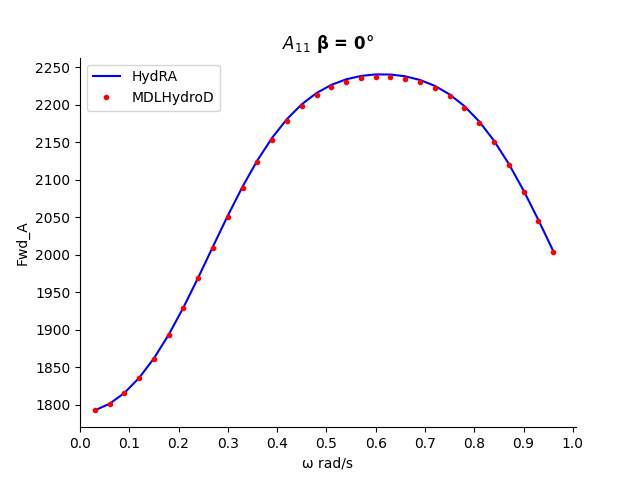
\includegraphics[width=\textwidth]{plots/kcs/added_mass/A11_BETA_0.png}
        \caption{$A_{22} \, \beta = 15^{\circ}$}
    \end{subfigure}
    \begin{subfigure}[b]{0.45\textwidth}
        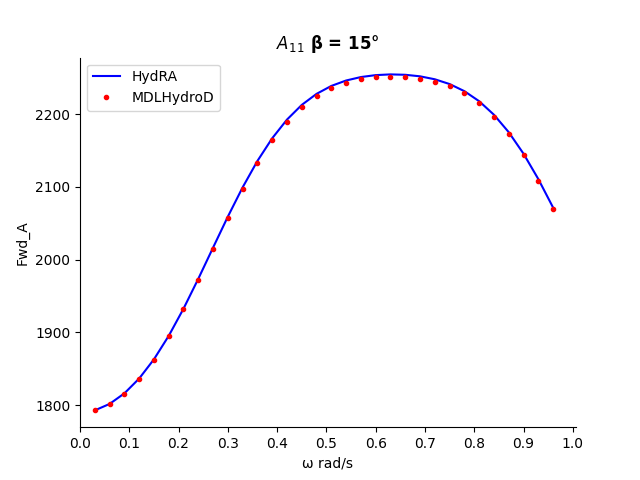
\includegraphics[width=\textwidth]{plots/kcs/added_mass/A11_BETA_15.png}
        \caption{$A_{22} \, \beta = 15^{\circ}$}
    \end{subfigure}
    \vspace{5pt}%
    \begin{subfigure}[b]{0.45\textwidth}
        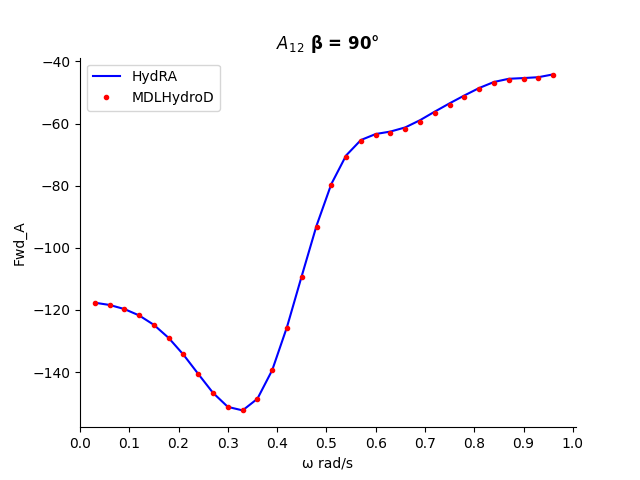
\includegraphics[width=\textwidth]{plots/kcs/added_mass/A12_BETA_90.png}
        \caption{$A_{11}\, \beta=0^{\circ}$}
    \end{subfigure}
    \begin{subfigure}[b]{0.45\textwidth}
        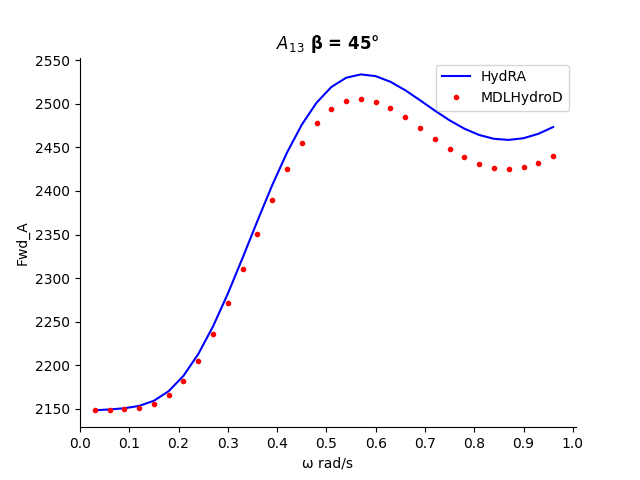
\includegraphics[width=\textwidth]{plots/kcs/added_mass/A13_ BETA_45.png}
        \caption{$A_{22} \, \beta = 11^{\circ}$}
    \end{subfigure}
    \vspace{5pt}%
    \begin{subfigure}[b]{0.45\textwidth}
        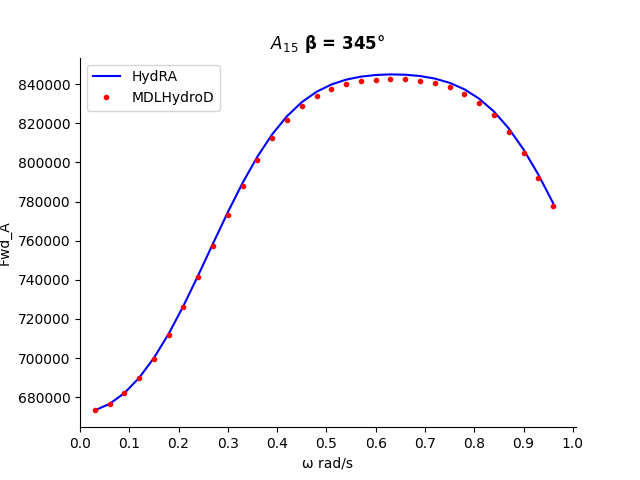
\includegraphics[width=\textwidth]{plots/kcs/added_mass/A15 _BETA_345.png}
        \caption{$A_{22} \, \beta = 12^{\circ}$}
    \end{subfigure}
    \begin{subfigure}[b]{0.45\textwidth}
        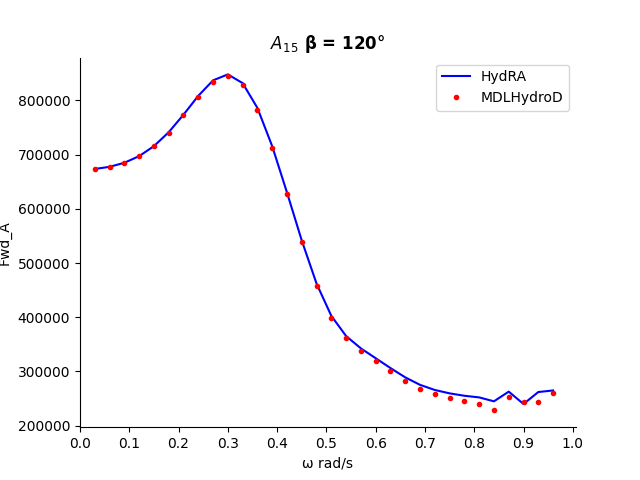
\includegraphics[width=\textwidth]{plots/kcs/added_mass/A15_BETA_120.png}
        \caption{$A_{22} \, \beta = 13^{\circ}$}
    \end{subfigure}
    \caption{KCS vessel added mass comparison - I}
    \label{fig:kcs_addedmass_1}
\end{figure}

\begin{figure}[H]
    \centering
    \ContinuedFloat
    \begin{subfigure}[b]{0.45\textwidth}
        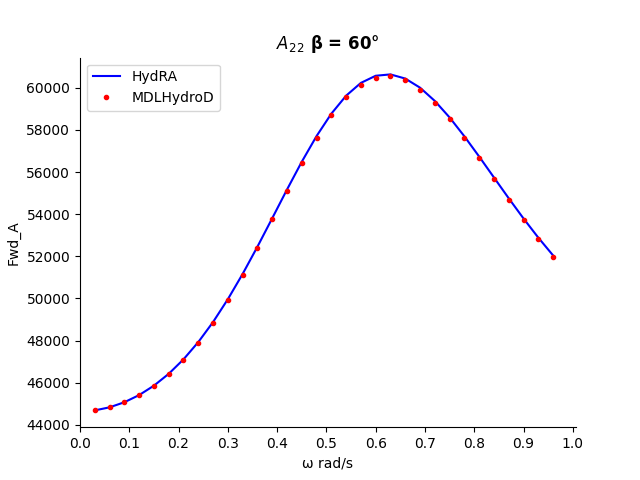
\includegraphics[width=\textwidth]{plots/kcs/added_mass/A22 _BETA_60.png}
        \caption{$A_{22} \, \beta = 14^{\circ}$}
    \end{subfigure}
    \begin{subfigure}[b]{0.45\textwidth}
        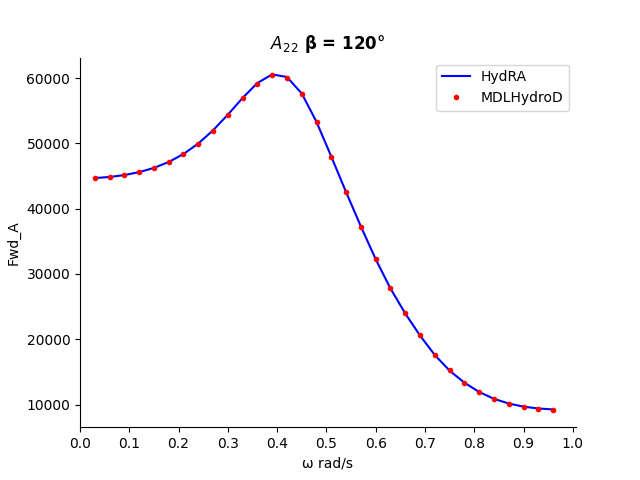
\includegraphics[width=\textwidth]{plots/kcs/added_mass/A22_BETA_120.png}
        \caption{$A_{22} \, \beta = 15^{\circ}$}
    \end{subfigure}
    \begin{subfigure}[b]{0.45\textwidth}
        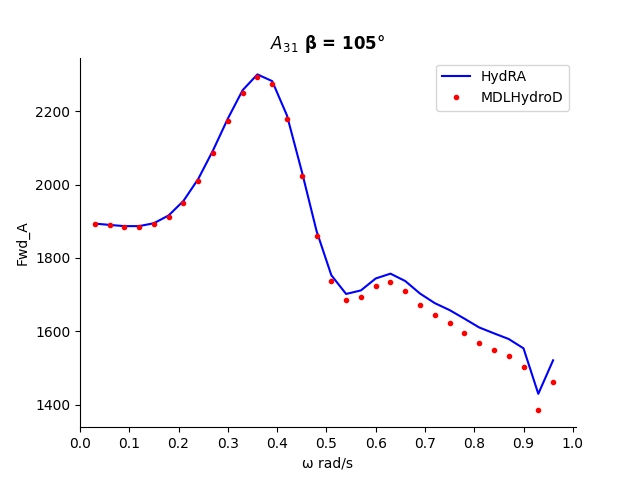
\includegraphics[width=\textwidth]{plots/kcs/added_mass/A31_BETA_105.png}
        \caption{$A_{22} \, \beta = 16^{\circ}$}
    \end{subfigure}
    \begin{subfigure}[b]{0.45\textwidth}
        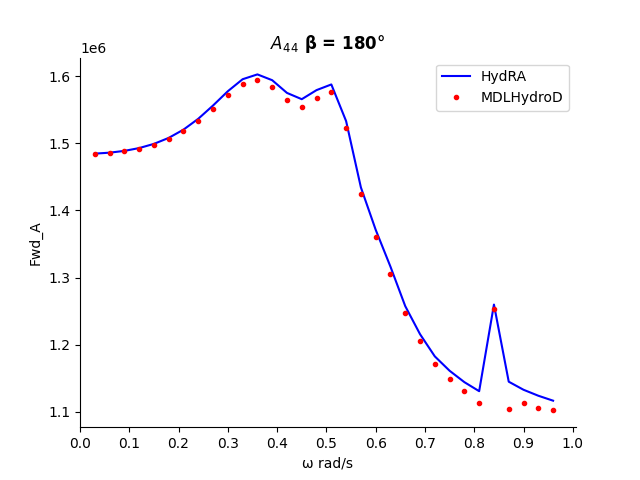
\includegraphics[width=\textwidth]{plots/kcs/added_mass/A44_BETA_180.png}
        \caption{$A_{22} \, \beta = 17^{\circ}$}
    \end{subfigure}
    \caption{KCS vessel added mass comparison - II}
    \label{fig:kcs_addedmass_2}
\end{figure}

\subsection{Radiation Damping}
\begin{figure}[H]
    \centering
    \begin{subfigure}[b]{0.45\textwidth}
        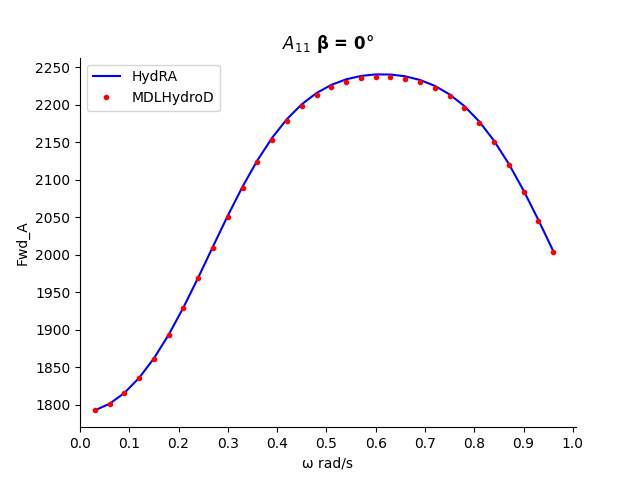
\includegraphics[width=\textwidth]{plots/kcs/added_mass/A11_BETA_0.png}
        \caption{$A_{11}\, \beta=0^{\circ}$}
    \end{subfigure}
    \begin{subfigure}[b]{0.45\textwidth}
        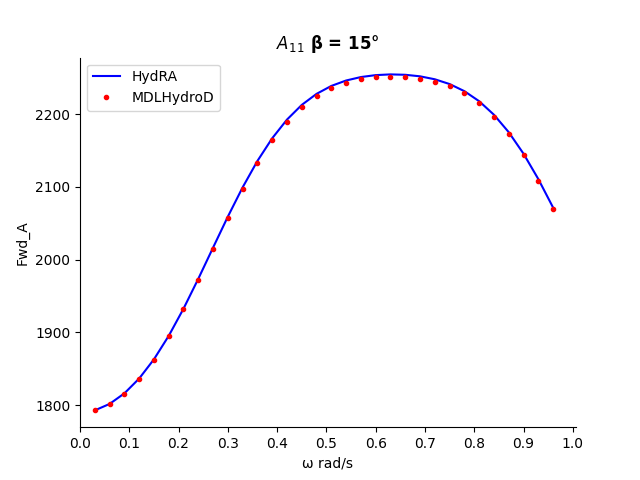
\includegraphics[width=\textwidth]{plots/kcs/added_mass/A11_BETA_15.png}
        \caption{$A_{22} \, \beta = 15^{\circ}$}
    \end{subfigure}
    % \caption{KCS vessel added mass comparison}
    \label{fig:kcs_addedmass_3}
\end{figure}
\subsection{Froude Krylov Force}
\begin{figure}[H]
    \centering
    \begin{subfigure}[b]{0.45\textwidth}
        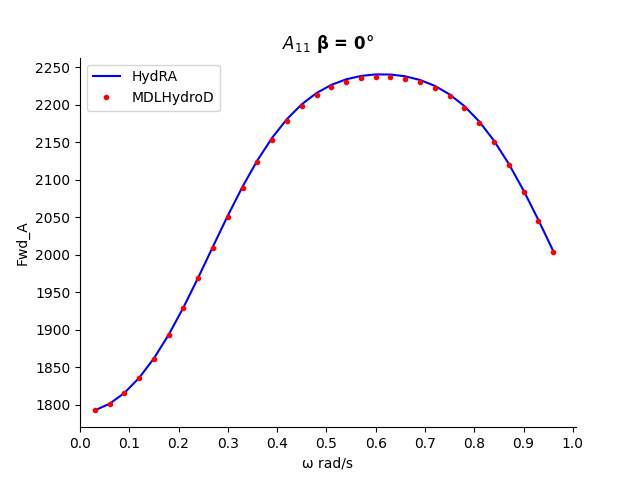
\includegraphics[width=\textwidth]{plots/kcs/added_mass/A11_BETA_0.png}
        \caption{$A_{11}\, \beta=0^{\circ}$}
    \end{subfigure}
    \begin{subfigure}[b]{0.45\textwidth}
        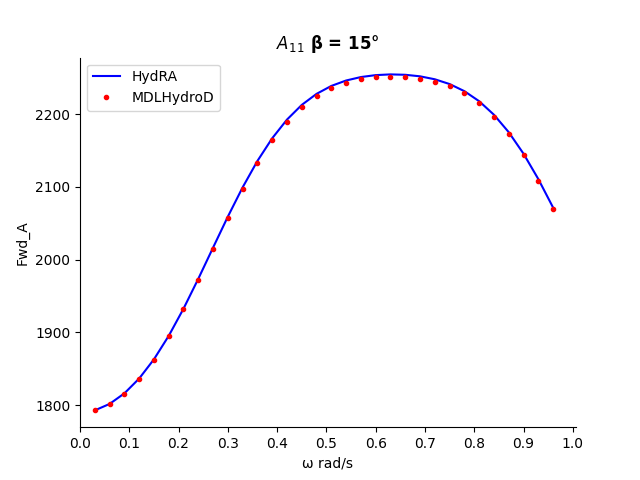
\includegraphics[width=\textwidth]{plots/kcs/added_mass/A11_BETA_15.png}
        \caption{$A_{22} \, \beta = 15^{\circ}$}
    \end{subfigure}
    % \caption{KCS vessel added mass comparison}
    \label{fig:kcs_addedmass_4}
\end{figure}
\subsection{Scattering Force}
\begin{figure}[H]
    \centering
    \begin{subfigure}[b]{0.45\textwidth}
        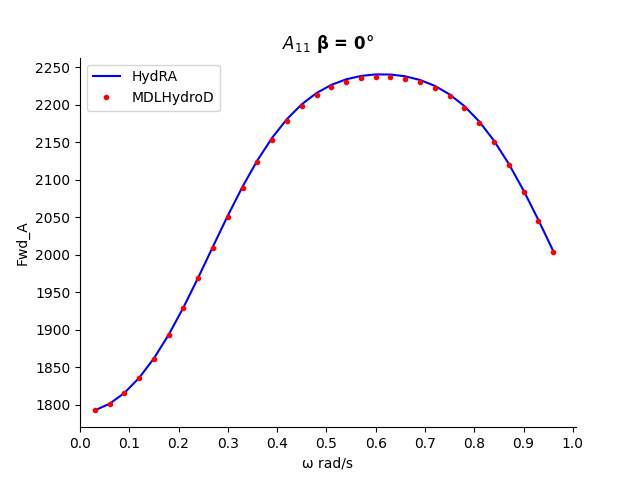
\includegraphics[width=\textwidth]{plots/kcs/added_mass/A11_BETA_0.png}
        \caption{$A_{11}\, \beta=0^{\circ}$}
    \end{subfigure}
    \begin{subfigure}[b]{0.45\textwidth}
        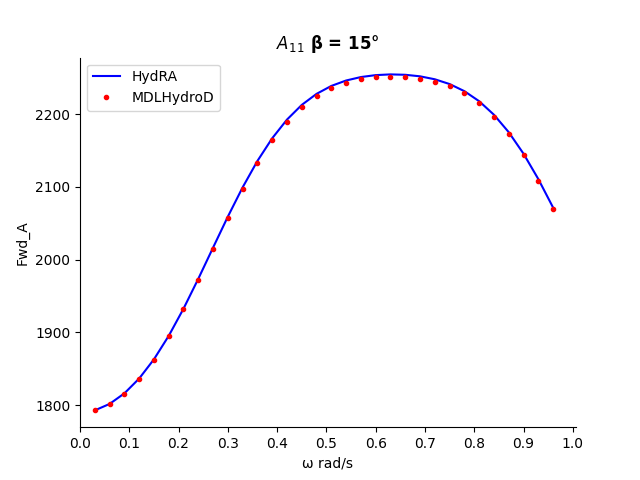
\includegraphics[width=\textwidth]{plots/kcs/added_mass/A11_BETA_15.png}
        \caption{$A_{22} \, \beta = 15^{\circ}$}
    \end{subfigure}
    % \caption{KCS vessel added mass comparison}
    \label{fig:kcs_addedmass_5}
\end{figure}

\section{KVLCC Vessel}
Input parameters for KVLCC2 are given in the following table.
\begin{table}[H]
    \centering
    \begin{tabular}{|c|c|}
        \hline
        parameter & value \\ 
        \hline
        \title{something}
        something & something \\
        something & something \\
        \hline
    \end{tabular}
    \caption{Parameters KCS vessel}
    \label{tab:kvlcc2_inp}
\end{table}